\documentclass[12pt,halfline,a4paper]{ouparticle}

\usepackage{booktabs}
\usepackage{xcolor}
\usepackage{graphicx}
\usepackage{caption}
\usepackage{subcaption}
\usepackage{cite}  % citeパッケージのインポート
\usepackage{natbib}  % 必要に応じて引用パッケージを使用
\bibliographystyle{apalike}

\begin{document}

\title{Does the Gender Employment Gap Expand Due to Natural Disasters? Evidence from the Great East Japan Earthquake}

\author{%
\name{Tomoto Masuda}
\address{}}

\abstract{This study examines the effects of the Great East Japan Earthquake of March 11, 2011, which led to a catastrophic tsunami and triggered a nuclear incident at Fukushima, on the gender employment gap in Fukushima Prefecture. Employing an event study approach alongside a difference-in-differences (DID) methodology with fixed effects regression, this study examines the earthquake's influence on gender-based employment dynamics. Drawing on extensive prefectural economic statistical data and individual socio-economic attributes from sources such as the Japan General Social Survey (JGSS), the Open Survey Data Japan Household Panel Survey on Consumer Preferences and Satisfaction (JHPS-CPS), the National Census, and the Housing and Land Survey, this study assesses the long-term effects of the earthquake on the gender employment gap. The results indicate that, in contrast to the immediate aftermath, the long-term impacts on the gender employment gap have attenuated significantly. This convergence can be attributed to multiple factors, including persistent governmental initiatives aimed at promoting female labor force participation, the economically rational adaptations of households in response to disruptions in community structures, and the possibility that the destruction of communities by the disaster also disrupted traditional gender norms and local gift economies, pushing women into the labor market.}

\date{\today}

\maketitle

\newpage

\tableofcontents

\newpage

\section{Introduction}
\label{sec1}

The impact of large-scale natural disasters on regional Gender Employment Gaps remain poorly understood, despite both being crucial policy concerns.

Previous studies present mixed findings on the impact of natural disasters on gender inequality, with some research indicating that such disasters widen gender gaps while other studies suggest a narrowing of these gaps. The Great East Japan Earthquake presented a unique opportunity to examine the dynamics of labor market responses to significant external shocks. This study focuses on Fukushima Prefecture, an area profoundly affected by both the earthquake and subsequent nuclear incident, to analyze the short-term and long-term impacts on the gender employment gap.

To frame the research question, this study aims to present a theoretical household model that encompasses four key elements. First, it considers household decision-making processes, where utility maximization drives choices about labor supply and participation. This model recognizes that households make complex decisions, balancing immediate needs with long-term economic rationality, often leading to gendered patterns of labor market engagement.

Secondly, the model incorporates the concept of economic shocks and adaptation mechanisms. The immediate aftermath of the disaster likely triggered rapid changes in employment patterns. However, over time, households develop adaptation strategies, including adjustments in labor supply preferences, acquisition of new skills, and reallocation of household labor responsibilities.

Thirdly, this study acknowledges the crucial role of government policies in shaping labor market outcomes. The theoretical framework examines how interventions aimed at promoting gender equality in employment can mitigate the adverse effects of economic shocks. This study assesses the effectiveness of these policies in both the short and long term, recognizing that policy impacts may evolve over time.

Lastly, the model considers the impact of community structure on household decision-making. The earthquake and its aftermath significantly disrupted local infrastructure and social networks, potentially altering the context in which households make employment decisions. Additionally, the destruction of traditional gender norms and local gift economies may have forced women into the labor market. I posit that long-term community rebuilding efforts can influence labor market dynamics and potentially reshape gender roles within households and the broader community.

By integrating these four elements - household decision-making, economic shocks and adaptation, policy interventions, and destruction of community - the theoretical model provides a comprehensive framework for understanding the complex interplay of factors affecting the gender employment gap in the wake of a major disaster.

\section{Background}
\label{sec2}

\subsection{The Great East Japan Earthquake }
\label{sec5.1}

 In Japan, the triple disaster of the Great East Japan Earthquake, the ensuing tsunami, and the Fukushima Daiichi nuclear crisis will have enduring implications on public perceptions of both local and national government authorities, as well as specialists in relevant fields. Furthermore, this disaster has profoundly reshaped attitudes towards nuclear energy, highlighting its risks and prompting widespread reconsideration of its role in Japan's energy strategy.


The Great East Japan Earthquake of March 2011 resulted in a tripartite catastrophe, comprising a magnitude 9.0 earthquake, a devastating tsunami, and a nuclear accident at the Fukushima Dai-ichi Nuclear Power plant. This disaster precipitated a severe humanitarian crisis, causing extensive damage particularly in the Iwate, Miyagi, and Fukushima prefectures in northeast Japan. According to the National Police Agency, 15,900 people lost their lives and 2,523 people remain unaccounted for, primarily as a result of the massive tsunami that struck the eastern coast of Japan. The affected prefectures account for 99.6\% of total fatalities and 99.8\% of total missing persons. In addition, a total of 3,784 fatalities and casualties were recognized as disaster-related deaths in Japan due to the exacerbation of chronic illnesses or suicide during evacuation. Approximately 90\% of fatalities were attributed to drowning. Table 1 presents a summary of the damages in the affected prefectures. The map below indicates the epicenter of the earthquake.

\begin{flushleft}
\begin{table}[h!]
  \caption{Direct Impact Overview in the Disaster-Stricken Prefectures}\label{table:disaster_situation}
  \begin{minipage}[c]{0.4\textwidth}
    \includegraphics[width=\textwidth,height=1.10\textwidth]{epicenter.jpeg}
  \end{minipage}
  \begin{minipage}[c]{0.48\textwidth}
    \raggedright
    \scalebox{0.8}{
    \begin{tabular}{|c|c|c|c|}
    \hline
    & \multicolumn{1}{c|}{Iwate} & \multicolumn{1}{c|}{Miyagi} & \multicolumn{1}{c|}{Fukushima} \\
    \hline
    Population & 1,330,147 & 2,348,165 & 2,029,064 \\
    Deceased & 4,675 & 9,544 & 1,614 \\
    Missing & 1,110 & 1,213 & 196 \\
    Fully destroyed houses & 20,185 & 83,932 & 20,136 \\
    Partially destroyed houses & 4,562 & 138,721 & 65,093 \\
    \hline
    \end{tabular}
    }
  \end{minipage}
\end{table}
\end{flushleft}

Fukushima Prefecture experienced a compound disaster involving both the tsunami triggered by the earthquake and the subsequent nuclear accident. The nuclear incident, in particular, necessitated large-scale evacuations, significantly disrupting local communities and labor markets. This unprecedented situation provides a unique context for examining the long-term socioeconomic impacts of compound disasters.

\subsection{Gender Gap in Japan}
\label{sec5.1}

According to the latest 2024 Global Gender Gap Report by the World Economic Forum (WEF), Japan ranks 118th out of 146 countries, placing it at the bottom among the G7 nations. Particularly, its rankings in the "Economic" and "Political" domains are notably low, with the "Economic" ranking being 120th out of 146 countries. Japan continues to exhibit substantial gender disparities in the economic sector, with the elimination of wage gaps remaining a significant challenge.

The ‘Act on Promotion of Women’s Participation and Advancement in the Workplace’ enacted in April 2016 has led to the development of an environment conducive to working women of child-rearing generations, with initiatives such as the introduction of a reduced working hours system, restrictions on overtime work, and the establishment of childcare facilities within companies. The Gender Equality Bureau of the Cabinet Office has also focused on supporting women in disaster-affected areas by addressing reconstruction efforts from a gender perspective, catering to the specific needs of women, and addressing child-rearing requirements.

\cite{Porcelli2019TheItaly} Porcelli and Trezzi (2018) conducted a counterfactual analysis using a balanced panel of 95 Italian provinces, examining the impact of 22 earthquakes on output and employment from 1986 to 2011. Their study, which compared affected provinces with similar neighboring provinces, revealed that the economic contraction following seismic events was generally minimal. In some instances, the net effect on output and employment was positive, as reconstruction activities outweighed the destruction of physical capital.



\section{Literature review}
\label{sec3}

Development economics models suggest an increase in household members’ labour supply as a shock-coping strategy which is associated with the narrowing of gender employment gaps. Several studies have documented a rise in female labor force participation following natural disasters. 


Some researchers, such as Canessa and Giannelli (2021), provide evidence that natural disasters spur women's labor force participation. They use georeferenced longitudinal household panel data to assess the impact of severe flooding in Bangladesh on women’s employment and empowerment, revealing a significant 13 percentage point increase in women's employment probability post-flood through a difference-in-differences analysis.


The study uses a difference-in-difference approach to compare changes in women’s labor outcomes in severely flooded villages to those in unaffected villages. The results indicate that the flooding led to a significant increase in female labor force participation. This increase is particularly prominent among women from lower-income households and those engaged in unpaid work on family farms who sought paid employment outside the household farm.


Income diversification: The flood negatively impacted household income, particularly from agriculture. As a result, women, especially those from poorer households, entered the workforce to mitigate income losses and support their families.
Increased bargaining power: Women who engaged in paid work outside the family farm experienced a notable increase in their decision-making power within their households. This finding aligns with the idea that earning an independent income empowers women and strengthens their position in intra-household negotiations.


On the other hand, in labor economics, the Risk Adjustment Hypothesis posits that during economic shocks or natural disasters, women are more susceptible to labor market exclusion and face higher risks of deteriorating work conditions or unemployment compared to men. This hypothesis suggests that specific labor market subgroups, particularly female and non-regular workers, often function as 'adjustment valves,' absorbing economic shocks. These groups are disproportionately affected, serving as mechanisms to mitigate broader economic impacts. This framework illuminates the gender-based disparities in employment stability and the uneven distribution of economic resilience across worker categories during crises. For instance, Kim, Ashley, and Corcoran (2014) examines the economic impact of the 2010 earthquake in Haiti, focusing on changes in household composition and employment retention. Authors found that the earthquake caused a significant reduction in employment rates, from 52.6\% prior to the earthquake to 28.6\% five months post-event. Gender disparities were evident, with only 34.2\% of women retaining their employment compared to 55.6\% of men. 


The study tries to fill gaps in the still sparse literature on the impact of natural disasters on gender disparities by differentiating between short-term and long-term effects, addressing the contradictory findings of existing research that suggests either an exacerbation or a reduction of gender gaps.


\section{Data and Descriptive Statistics}
\label{sec4}


\subsection{Employment Situation in Fukushima Prefecture}
\label{sec4.1}

The employment and unemployment landscape in fiscal year 2011 was severely impacted by the Great East Japan Earthquake on March 11, 2011. The earthquake and subsequent tsunami, coupled with the severe nuclear incident at the Fukushima Daiichi Nuclear Power Plant, led to business closures, mass evacuation of residents both within and outside the prefecture, and reputational damage. These factors resulted in an exceptionally grave employment situation. Initially, there was a sharp increase in job seekers and unemployment insurance recipients. However, the employment situation gradually improved, primarily due to an upsurge in job openings related to post-disaster reconstruction, particularly in the construction sector. Consequently, the monthly effective job openings-to-applicants ratio rose to 0.70 in November 2011, surpassing the national average of 0.69 for the first time in 10 years and 6 months.


\subsection{Microdata sets}
\label{sec4.1}

To elucidate the causal relationship and mechanisms through which the Great East Japan Earthquake affected the Gender Employment Gap in the disaster-affected regions, this study emphasizes the necessity of analyzing not only regional-level economic statistical panel data but also individual-level microdata pertaining to various socio-economic attributes. The microdata sets employed in this study include:

\subsection{Regional data analysis}
\label{sec4.1}

Figure 1 illustrates the number of new job openings-to-applicants ratio recorded at Hello Work, Japan’s public employment security office, which maintains a comprehensive database of current job vacancies accessible to all citizens. 

\begin{figure}[h!]
    \centering
    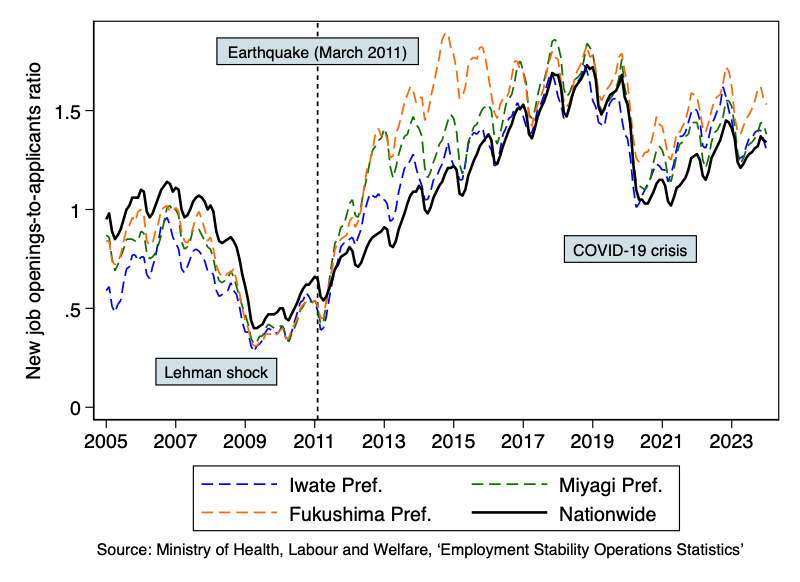
\includegraphics[width=0.9\textwidth]{New job openings-to-applicants ratio.png}  % 幅を本文の80%に設定
    \caption{New job openings-to-applicants ratio}
    \label{fig:new_job_openings}
\end{figure}

Although the number of job openings in the three disaster-affected prefectures of Iwate, Miyagi, and Fukushima initially decreased significantly immediately after the disaster, they have since outperformed the national average. This improvement is largely attributed to the reconstruction demand, including a surge in the construction industry. The first research question of this study investigates how the gender employment gap has evolved under such circumstances.

\newpage

Figure 2 shows a long-term trend of the proportion of women job seekers among total new job applications submitted to Hello Work in Fukushima Prefecture. A higher proportion suggests a narrowing gender employment gap. 

\begin{figure}[h!]
    \centering
    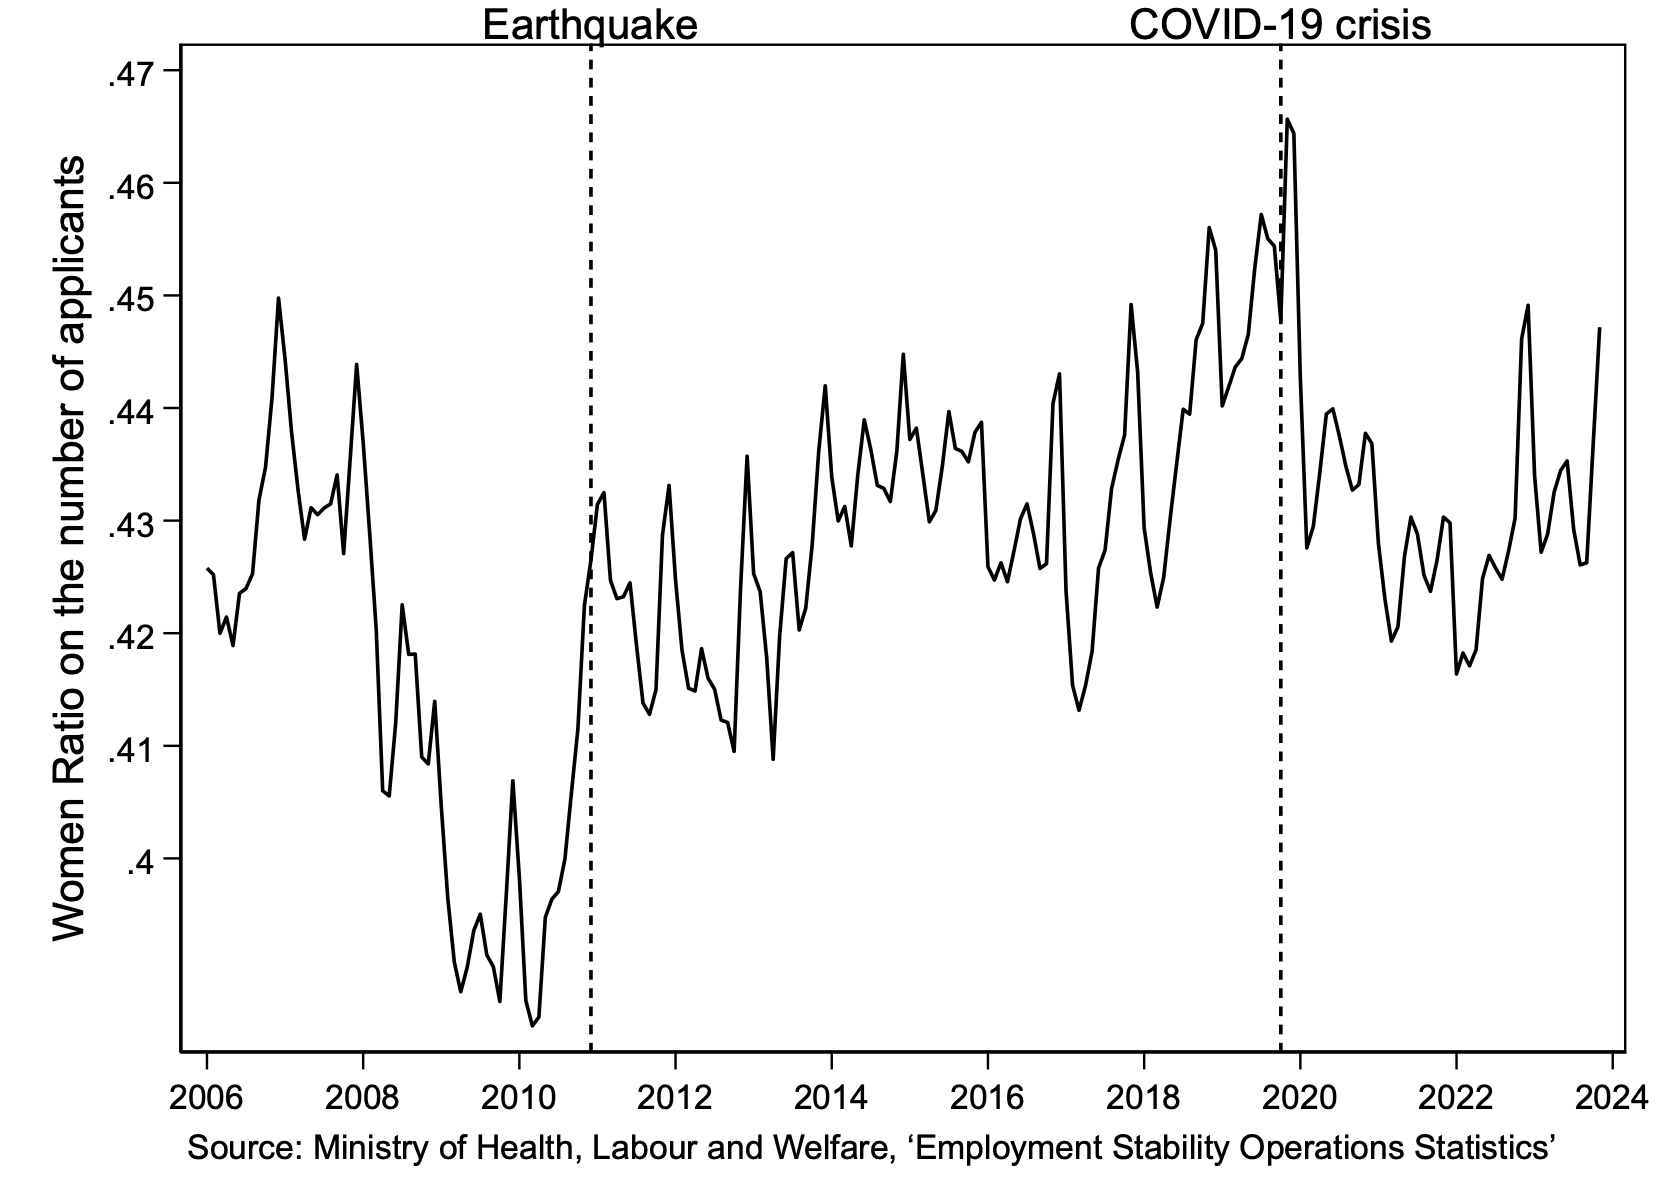
\includegraphics[width=0.9\textwidth]{Women ratio on the number of applicants in Fukushima2.jpeg}  % 幅を本文の80%に設定
    \caption{Women ratio on the number of applicants in Fukushima Pref.}
    \label{fig:women_ratio_fukushima}
\end{figure}

\newpage

The graph reveals that in Fukushima Prefecture, prior to the disaster, from 2008 to the earthquake, the proportion of male job seekers had increased due to the impact of the Lehman Shock. However, post-disaster, there has been a gradual increase in the proportion of female job seekers. In the disaster-affected areas, there is a potential long-term trend of increasing female labor force participation.

\newpage

Figure 3 presents a time-series graph showing the proportion of active women job seekers among total job applications submitted to Hello Work in Fukushima Prefecture.

\begin{figure}[h!]
    \centering
    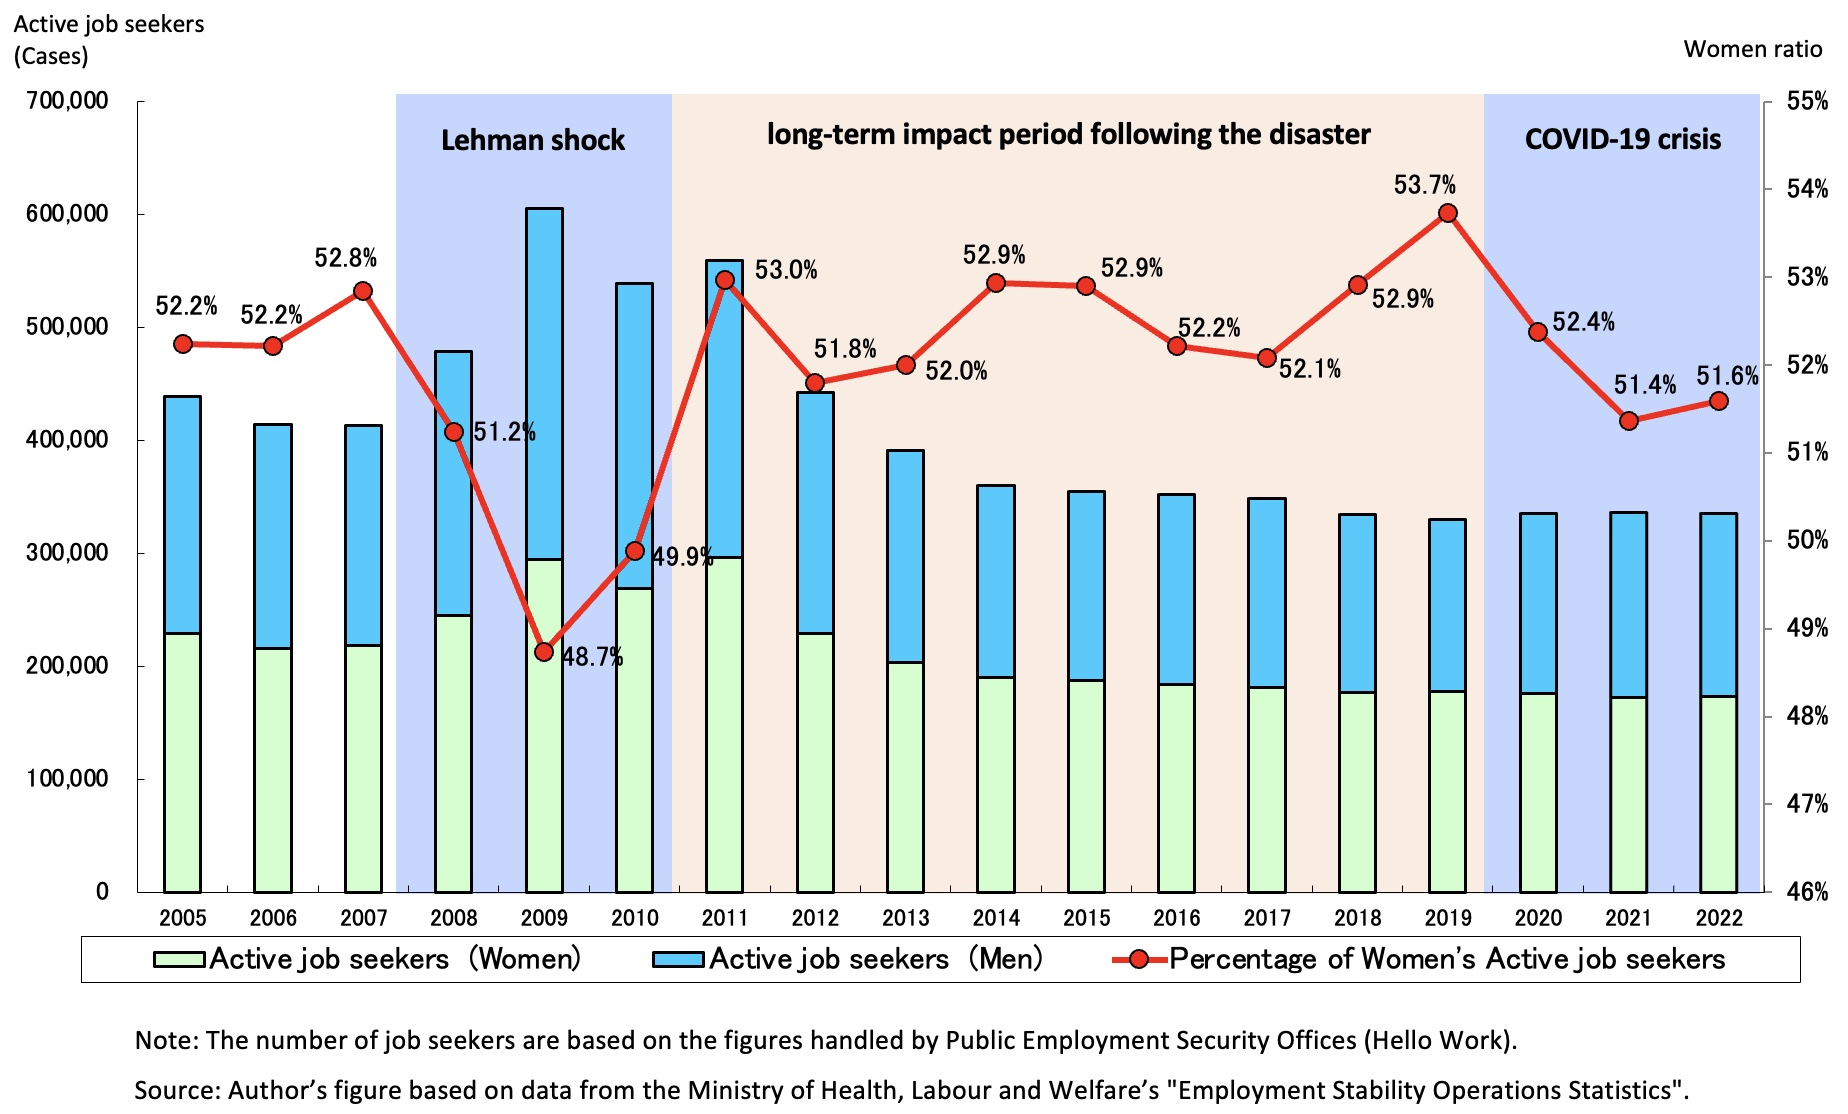
\includegraphics[width=0.9\textwidth]{Women ratio on the number of active job seekers2}  % 幅を本文の80%に設定
    \caption{Women ratio on the number of active job seekers in Fukushima Pref.}
    \label{fig:women_ratio_fukushima}
\end{figure}

Labor market trends in Fukushima Prefecture over the past two decades reveal three distinct phases. During the 2008-2010 global financial crisis, the proportion of female job seekers decreased, suggesting a greater impact on male employment. Following the 2011 Great East Japan Earthquake, there was a sustained increase in the proportion of female job seekers, a trend that persisted throughout the post-disaster period. Since 2020, the COVID-19 pandemic has resulted in a slight decline in the female share of job seekers, potentially indicating a shift in labor market dynamics.

\newpage

Figure 4 illustrates both short-term (upper graph) and long-term (lower graph) changes in unemployment insurance recipients in Fukushima Prefecture following the Earthquake. Regarding short-term effects, while overall recipient numbers spiked briefly before returning to pre-disaster levels within a year, the proportion of female recipients also showed a notable increase. This percentage rose from 52-53\% pre-disaster to a peak of 57.2\% in August 2011, five months post-earthquake, before gradually declining. Notably, this peak was 1.7 percentage points higher than the nationwide figure. This trend aligns with reports of heightened short-term employment challenges for women, particularly in heavily impacted coastal areas where female-dominated industries like seafood processing, which employed many part-time women workers, suffered significant damage. Conversely, long-term effects reveal a contrasting trend, with the proportion of female recipients in Fukushima declining relative to the national average. This disparity reached its maximum in 2017, with Fukushima's 55.4\% being 4.7 percentage points lower than the nationwide figure of 60.1\%.


\begin{figure}[h!]
    \centering
    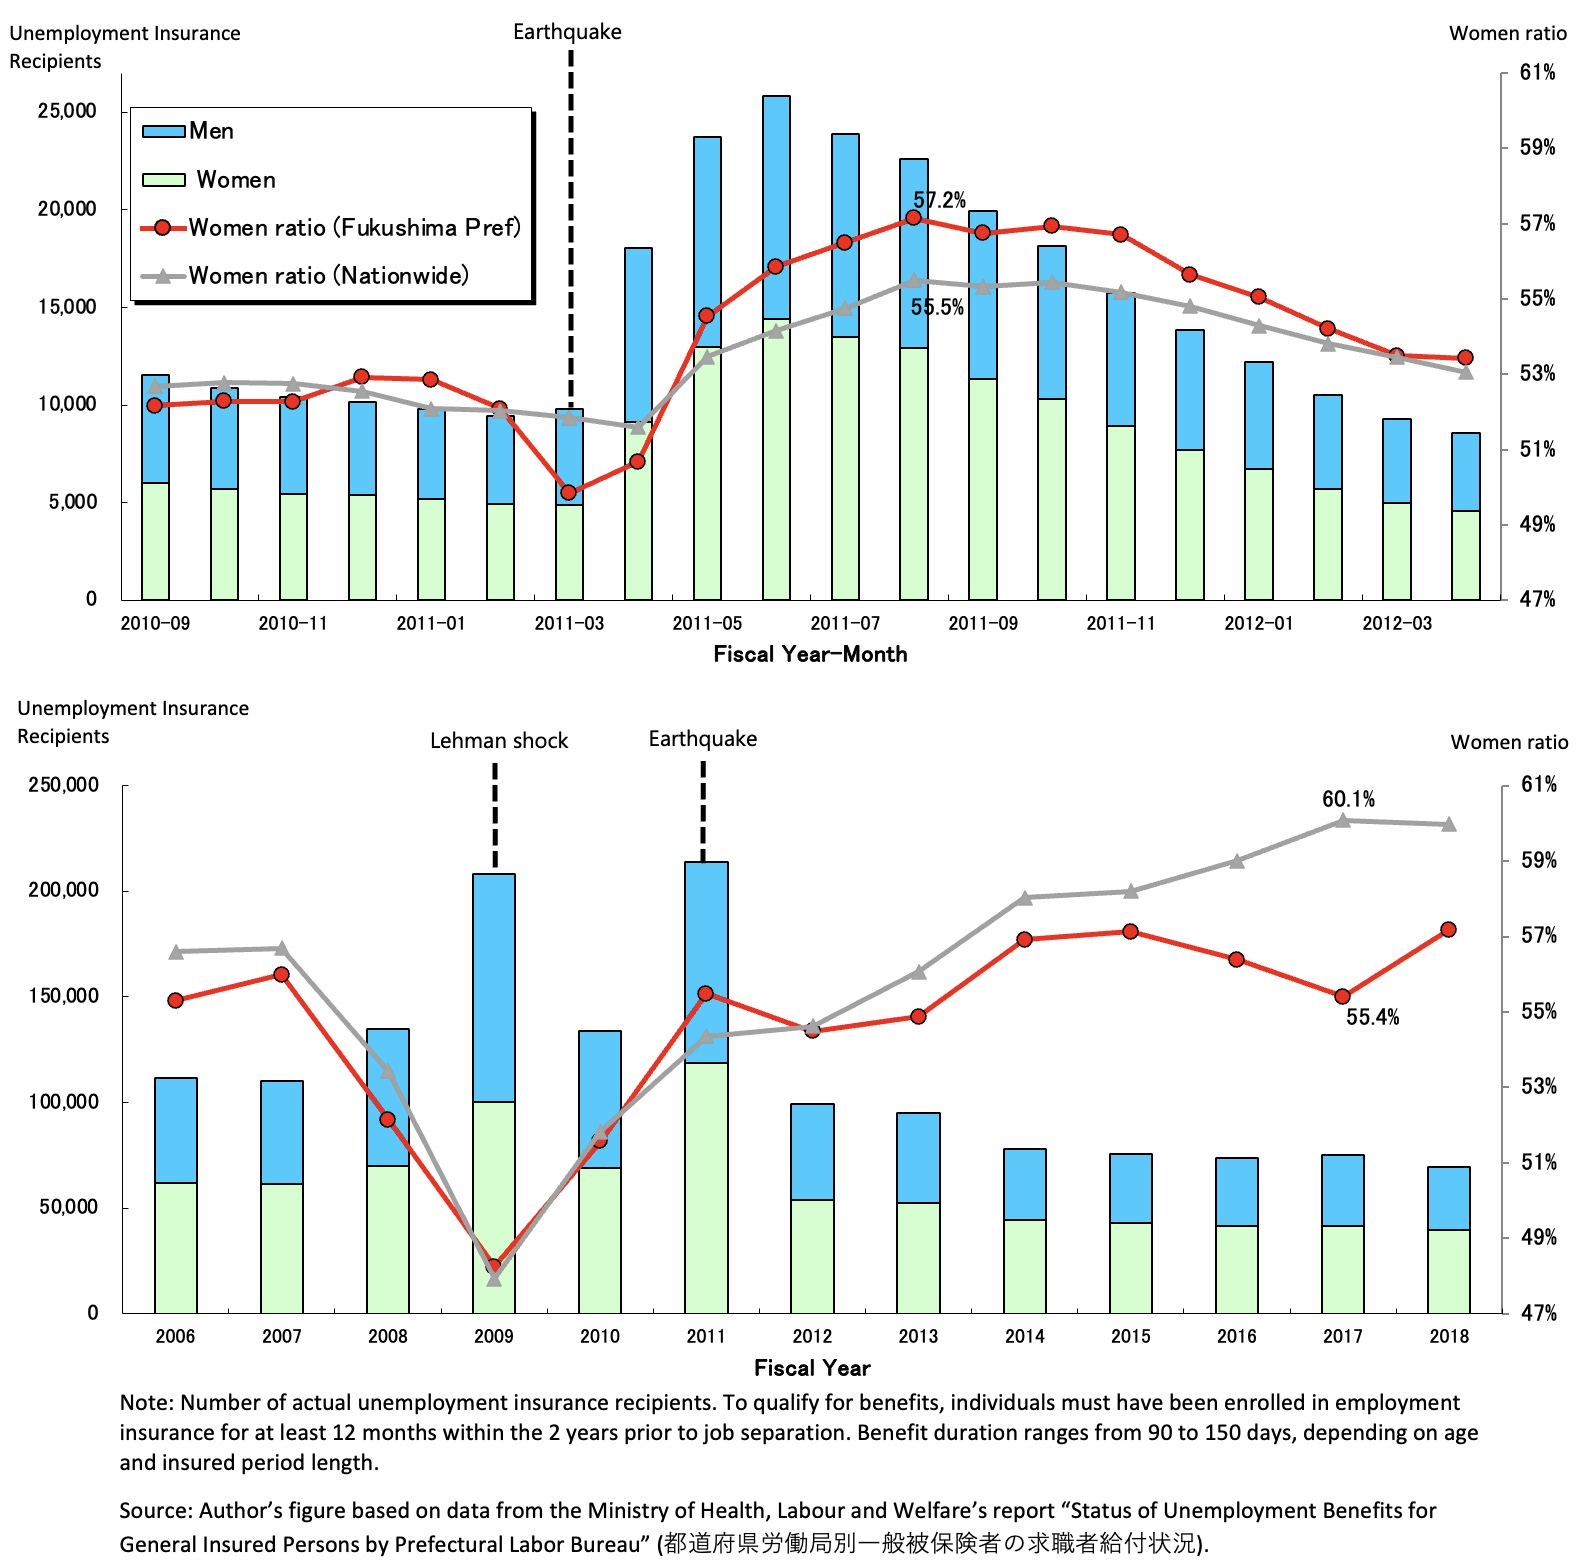
\includegraphics[width=0.9\textwidth]{Number of Actual Unemployment Insurance Recipients2.jpeg}  % 幅を本文の80%に設定
    \caption{Women ratio on the number of Unemployment Insurance Recipients in Fukushima Pref.}
    \label{fig:women_ratio_fukushima}
\end{figure}



Figure 5 presents a line graph illustrating the number of applicants for public unemployment insurance (Employment Insurance) in Fukushima Prefecture, along with the proportion of female applicants relative to total applicants. The graph also includes the national average for comparison. 

\begin{figure}[h!]
    \centering
    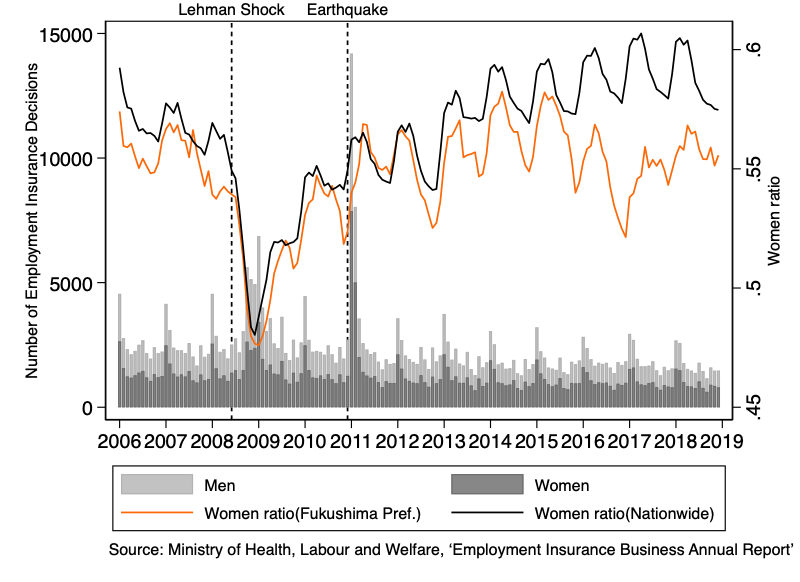
\includegraphics[width=0.9\textwidth]{Number of Employment Insurance Decisions_2.png}  % 幅を本文の80%に設定
    \caption{Number of Employment Insurance Decisions by Gender in Fukushima Pref.}
    \label{fig:employment_insurance_decisions}
\end{figure}

From this graph, it is evident that in Fukushima Prefecture, the proportion of female applicants for unemployment insurance has shown a declining trend post-disaster. This suggests a potential improvement in the labor market conditions for female workers in the disaster-affected areas over the longer term.

\newpage

\subsection{Data sets}
\label{sec5.1}

To study the effects of the triple tragedy of the earthquake, tsunami, and nuclear disaster and the theoretical predictions, I construct a monthly panel of 47 Japanese prefectures running from 2000 to 2018(just before COVID-19 pandemic).


This study uses a panel data of 65 countries observed over the 1987 to 2021 period. 

To elucidate the causal relationship and mechanisms through which the Great East Japan Earthquake affected the Gender Employment Gap in the disaster-affected regions, this study emphasizes the necessity of analyzing not only regional-level economic statistical panel data but also individual-level microdata pertaining to various socio-economic attributes. The microdatasets employed in this study include:

\begin{table}[h]
    \centering
    \caption{Individual-level Surveys}
    \label{tab:annual_income}
    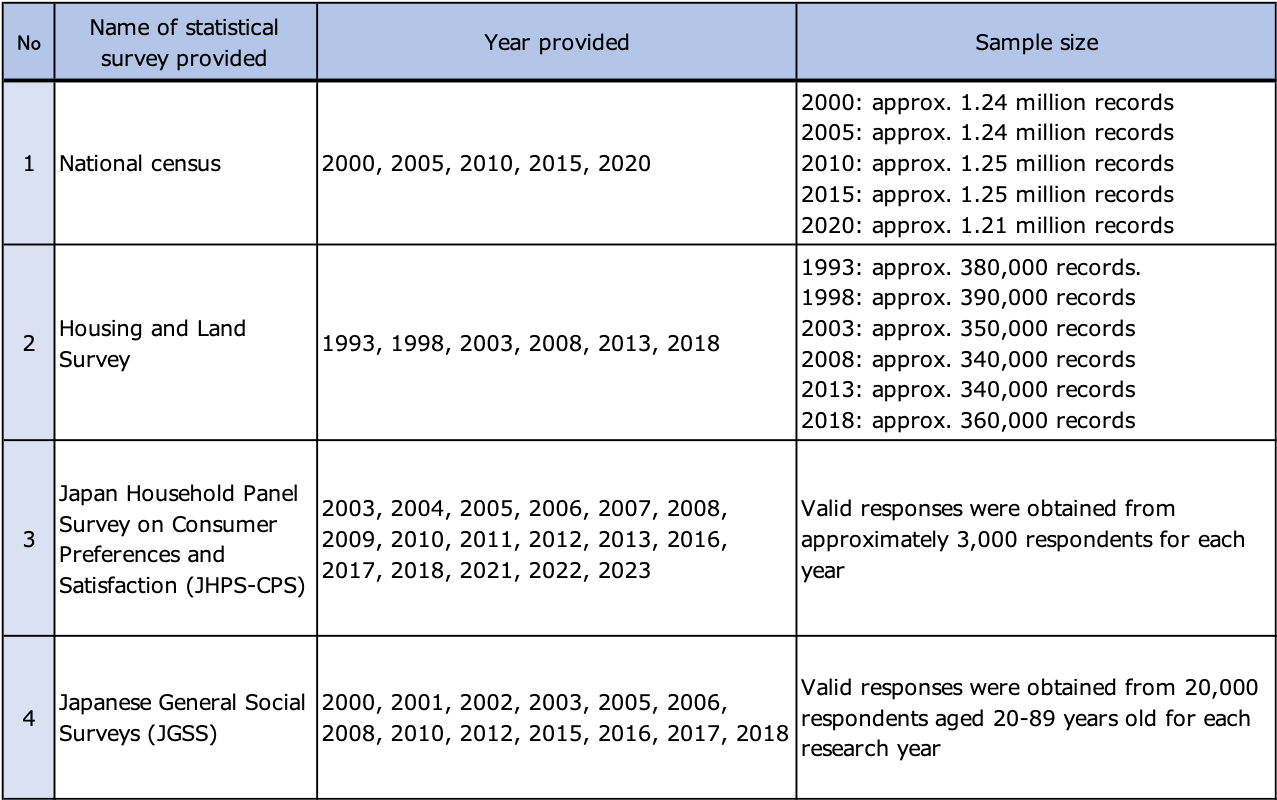
\includegraphics[width=0.9\textwidth]{Statistical surveys.png}  % 幅を本文の80%に設定
\end{table}

\newpage

\subsection{Empirical Strategy}
\label{sec5.1}

Over the next few chapters, I will cover some recent developments in DID methods. 


This study statistically estimates whether trends similar to those observed at the regional level in microdata can be identified using four anonymized individual-level datasets: the Japan General Social Survey (JGSS), the Open Survey Data Japan Household Panel Survey on Consumer Preferences and Satisfaction (JHPS-CPS), the National Census, and the Housing and Land Survey. The analysis employs a Difference-in-Differences (DID) approach with Fukushima Prefecture as the Treatment group and other prefectures as the Control group.

The empirical strategy of this study employs the difference-in-differences (DID) methodology. For the implementation of the Difference-in-Differences (DiD) analysis, I employ a pooled DiD methodology, which is particularly suitable for non-continuous time series data, such as quinquennial census surveys. This approach involves aggregating data into two distinct periods: pre-earthquake and post-earthquake. In cases where continuous annual data is unavailable, this method allows for the bifurcation of the dataset into these two critical temporal segments. By doing so, I can estimate the average treatment effect across the aggregated pre-treatment and post-treatment periods, effectively capturing the impact of the seismic event despite the temporal gaps in data collection. This strategy is especially advantageous when dealing with infrequently collected cross-sectional data, as it maximizes the utilization of available information while adhering to the fundamental principles of DiD analysis.

The econometric model is specified as follows:

\begin{equation}
Y_{ipt} = \alpha_{p} + \beta D_{p} + \eta Post_{t} + \gamma (D_{pt} * Post_{t}) + X_{ipt} + \epsilon_{ipt}
\end{equation}

Here, \( Y_{idt} \) denotes the outcome variable, such as the employment rate, annual income, or working hours, for individual \( i \) in prefecture \( p \) at year \( t \). \( \gamma \) represents the disasters effect that I aim to estimate. 


\begin{equation}
\begin{aligned}
E[\text{DiD estimator}] \\
&= (E[Y_{ipt}|D_i = 1, \text{Post}_t = 1] - E[Y_{ipt}|D_i = 1, \text{Post}_t = 0]) \\
&- (E[Y_{ipt}|D_i = 0, \text{Post}_t = 1] - E[Y_{ipt}|D_i = 0, \text{Post}_t = 0]) \\
&= (\alpha_{p} + \beta + \eta + \gamma - \beta_0 - \beta) - (\alpha_{p} + \eta - \alpha_{p}) \\
&= \gamma
\end{aligned}
\end{equation}





ーーーーーーーーーーーーー

To adequately capture the dynamic effects of natural disasters, which inherently have long-term and evolving impacts, I employ a Two-Way Fixed Effects Event Study (TWFE Event Study) approach. This method extends the traditional Difference-in-Differences (DiD) framework to account for the temporal dimension of disaster impacts. The model is specified as follows:

\begin{equation}
Y_{ipt} = \beta_ip + \eta_t + \sum_{l}^{} \gamma_l 1 [t-s_{pt} = l] + \epsilon_{ipt}
\end{equation}

Where: \\
$Y_{ipt}$ is the outcome variable for individual \( i \) in prefecture \( p \) at year \( t \) \\
$\beta_ip$ represents unit fixed effects for individual \( i \) in prefecture \( p \) \\
$\eta_t$ denotes time fixed effects \\
$s_{i}$ is the timing of the earthquake occurrence \\
$l$ is the number of periods relative to the earthquake
$\gamma_l$ captures the effect of the disaster $l$ periods after (or before) its occurrence \\
$\epsilon_{ipt}$ is the error term

This specification allows for estimating the dynamic treatment effects over an extended period, both pre- and post-disaster, thereby providing a comprehensive understanding of the disaster's evolving impact on economic outcomes.

ーーーーーーーーーーーーー





Using individual-level data from the Japanese General Social Surveys (JGSS), I investigate changes in individual annual income by gender between the three disaster-affected prefectures and other prefectures before and after the earthquake. The JGSS dataset consists of cross-sectional data collected in 2000, 2001, 2002, 2003, 2005, 2006, 2008, 2010, 2012, 2015, 2016, 2017, and 2018, provided by the JGSS Research Center at Osaka University of Commerce. This survey includes responses from over 20,000 individuals aged 20 to 89 who completed self-administered questionnaires. 

Using pooled DID analysis methodology, I present the results in Figure 4, which indicate a statistically significant increase in income among women in the disaster-affected prefectures when comparing the periods before (2000 to 2010) and after (2012 to 2018) the earthquake, over a sufficiently long-term horizon.


\begin{figure}[h!]
    \centering
    \includegraphics[width=0.9\textwidth]{Kernel density graphs of respondent’s annual income from main job.png}  % 幅を本文の80%に設定
    \caption{Kernel density graphs of respondent’s annual income from main job (Income bands, N= 20,119)}
    \label{fig:conceptual_model}
\end{figure}

The pre/post income band difference for affected prefecture women was statistically significant (Table 3; T-value: -1.849, P-value: 0.065). As Figure 4 and Table 3 shows, only this ‘Women in affected prefectures’ group's average income bands shifted right (increased) pre/post-disaster.


\begin{table}[h!]
    \centering
    \caption{Mean of annual income: Pre/Post-disaster period (Income bands, N=20,119)}
    \label{tab:annual_income}
    
\includegraphics[width=0.9\textwidth]{Annual income table.png}  % 幅を本文の80%に設定
\end{table}

\newpage

\section{Conclusion}
\label{sec5}

\subsection{Regional level}
\label{sec5.1}

The case of the Great East Japan Earthquake illustrates the complexity of the reconstruction process and rational household responses when communities are disrupted by both tsunami disasters and nuclear accidents. This study presents changes in gender gaps in such complex disaster-affected areas as a conceptual model, as depicted in Figure 5.


At Phase 1, an exogenous shock would alter the production function of both sellers and buyers, disproportionately affecting female employment due to the higher prevalence of non-regular workers among women.

At Phase 2, the female employment recovery rate would surpass that of males, driven by three factors: the reconstruction demand boom, household shock coping strategies necessitating women to seek employment, and government policies aimed at promoting employment opportunities for women.

At Phase 3, in the long term, the impact of the disaster gradually diminishes, and the employment levels of women in the affected areas converge towards the national average.


\begin{figure}[h!]
    \centering
    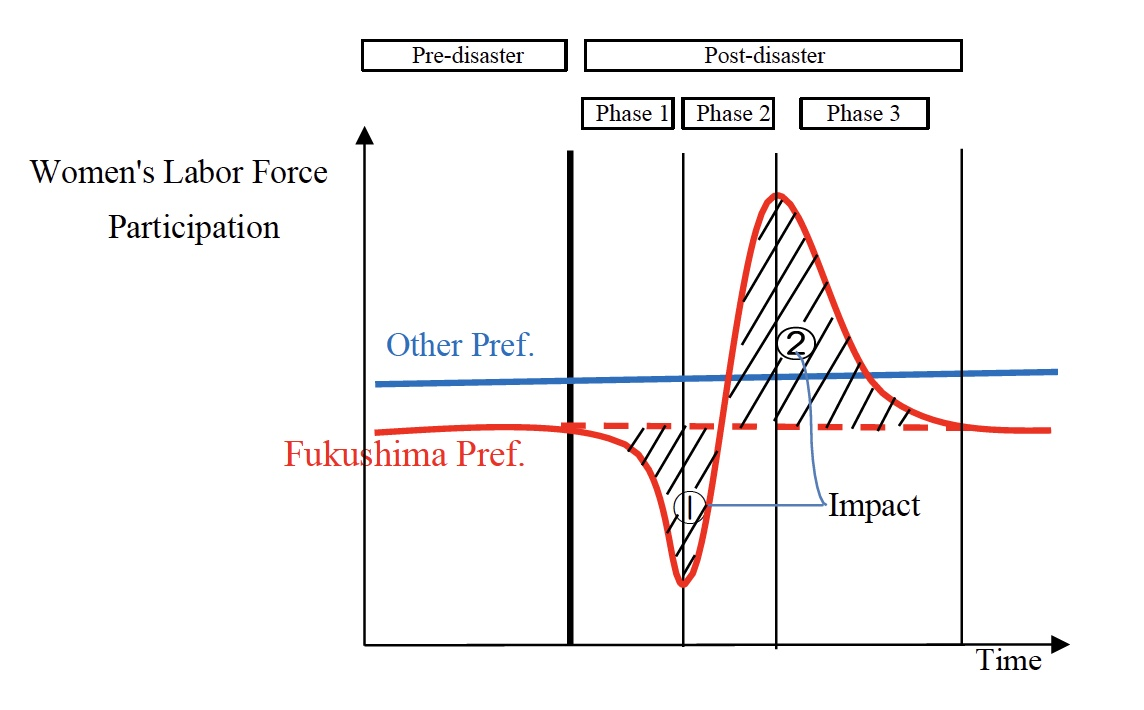
\includegraphics[width=0.9\textwidth]{A conceptual model.jpeg}  % 幅を本文の80%に設定
    \caption{A conceptual model of long-term effects on Women's Labor Force Participation}
    \label{fig:conceptual_model}
\end{figure}

Initially, these events disproportionately impacted women workers negatively. However, The earthquake and nuclear disaster potentially accelerated women's labor market participation by fundamentally disrupting communities bound by traditional gender roles. In the short term, the disaster and nuclear accident had a more severe negative impact on female workers. However, in the long term, this catastrophic event, while devastating, may have inadvertently challenged long-standing societal norms, thus facilitating increased female workforce engagement.

\newpage

\subsection{Household level}
\label{sec5.1}

This study models how households made economically rational decisions following the Great East Japan Earthquake by utilizing a microdata-based DID analysis, which supports the gender employment gaps identified in regional-level statistical data. This household model suggests that the destruction of communities by the earthquake also disrupted traditional gender norms and local gift economies, potentially forcing women into the labor market.


\subsection{Theoretical model}
\label{sec5.1}

This study constructs a household decision-making model to elucidate the fluctuations in female employment before and after a major earthquake. The model draws upon the agricultural household model framework (Huffman \& El-Osta, 1997; Omamo, 1998; Key, Sadoulet, \& Janvry, 2000), adapting it to the context of disaster-affected urban and rural areas. It incorporates elements from development economics, which suggest an increase in household members' labour supply as a shock-coping strategy.
The model delineates three distinct phases: the immediate aftermath, the recovery period, and the long-term equilibrium. In Phase 1, it accounts for the exogenous shock's impact on production functions and the disproportionate effect on female employment due to the prevalence of non-regular work among women. Phase 2 captures the interplay between reconstruction demand, household coping strategies necessitating female employment, and government policies promoting women's work opportunities. Finally, Phase 3 models the gradual convergence of female employment levels in affected areas towards the national average as the disaster's impact wanes over time.
By integrating these elements, the model aims to provide a comprehensive framework for analyzing the dynamics of female labor force participation and intra-household bargaining power in the wake of a major natural disaster.



% すべての文献を引用リストに追加
\nocite{*}

% 参考文献リストの場所を示す
\bibliography{references}  % 'references.bib'ファイルの名前を指定
\bibliographystyle{plain}  % 引用スタイルを指定


\end{document}
